\documentclass[lang=cn,11pt,a4paper,cite=authornum]{paper}

\title{编译原理与技术 实验一:词法分析程序的设计与实现 \\ 实验报告}
\author{毛子恒 \\ 2019211397}
\institute{北京邮电大学\ 计算机学院}

\date{\zhtoday}

% 本文档命令
\usepackage{array}
\newcommand{\ccr}[1]{\makecell{{\color{#1}\rule{1cm}{1cm}}}}
\nocite{*}

\begin{document}

\maketitle

\section{概览}

\subsection{任务描述}

设计并实现C语言的词法分析程序,要求如下。

\begin{enumerate}
    \item 可以识别出用C语言编写的源程序中的每个单词符号,并以记号的形式输出每个单词符号。
    \item 可以识别并跳过源程序中的注释。
    \item 可以统计源程序汇总的语句行数、单词个数和字符个数,并输出统计结果。
    \item 检查源程序中存在的错误,并可以报告错误所在的位置。
    \item 发现源程序中存在的错误后,进行适当的恢复,使词法分析可以继续进行,对源程序进行一次扫描,即可检查并报告出源程序中存在的词法错误。
\end{enumerate}

采用C++作为实现语言,手工编写词法分析程序。

\subsection{开发环境}

\begin{itemize}
    \item macOS Big Sur 11.6
    \item Apple clang version 12.0.5
    \item cmake version 3.19.6
    \item Clion 2021.2.1
    \item Visual Studio Code 1.60.2
\end{itemize}

\section{模块介绍}

\subsection{模块划分}

各模块及其关系如\figref{fig:structure}。

\begin{figure}[htbp]

    \centering
    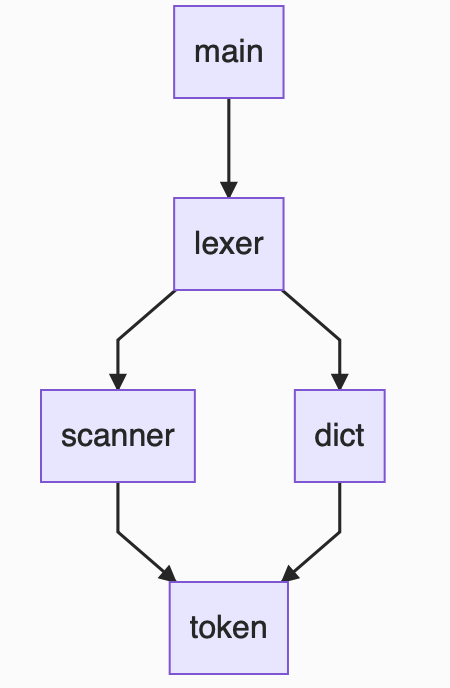
\includegraphics[width=0.25\linewidth]{./images/structure.png}
    \caption{模块关系图\label{fig:structure}}

\end{figure}

其中,\mintinline{text}{token}模块定义了记号的数据结构;\mintinline{text}{dict}模块定义了用于快速检索关键字的字典树;\mintinline{text}{scanner}模块对文件输入流进行简单封装,实现了一个简单的缓冲区,实现向前预先查看数个字符的功能;\mintinline{text}{lexer}模块是词法分析器,将文件流中的字符分成不同的记号,并用数据结构表示。

\subsection{记号数据结构}

在编写词法分析程序时,我参考了ISO/IEC 9899:1999标准,在标准的6.4节中有对词法单元的详细规定。我在标准的基础上做了一些改动:

\begin{enumerate}
    \item 将满足以下条件的部分标记为预处理器,预处理器部分不作处理。
          \begin{itemize}
              \item 以\mintinline{text}{#}开头,且此符号在行首或者此符号前都是空白字符。
              \item 以换行结束,除非忽略本行末尾的空白字符后本行末尾的最后一个字符为\mintinline{text}{\}。
          \end{itemize}
    \item 将在程序中其他地方出现的\mintinline{text}{#}和\mintinline{text}{##}符号视为非法符号。
    \item 不处理Universal character。
\end{enumerate}

我将记号分为以下十类:

\begin{enumerate}
    \item Unknown,未识别和出现错误的记号,本词法分析器能够识别出如下几种错误:
          \begin{itemize}
              \item 非法的\mintinline{text}{#}和\mintinline{text}{##}符号。
              \item 未知的符号。
              \item 未闭合的块注释。
              \item 不合法的数字。
              \item 未闭合的字符常量。
              \item 未闭合的字符串字面值。
              \item Slash Newline at EOF,在字符常量、字符串字面值或者预处理器中,出现\mintinline{text}{\}符号后,直到EOF也没有新的行。
          \end{itemize}
    \item Keyword,关键字,在C99标准中共37个。
    \item Identifier,标识符。
    \item Integer Constant,整数常量。
    \item Float Constant,浮点数常量。
    \item Char Constant,字符常量。
    \item String Literal,字符串字面值。
    \item Punctuator,标点符号,在C99标准中共49个。
    \item Preprocessing,预处理器。
    \item EOF,文件末尾。
\end{enumerate}

\subsubsection{TokenLocation}

此类用于存储一个记号的位置。

\begin{code}
    \begin{minted}{C++}
class TokenLocation
{
public:
    TokenLocation();
    TokenLocation(std::string file_name_, unsigned int row_, unsigned int column_);
    friend std::ostream &operator<<(std::ostream &os, const TokenLocation &location);
private:
    std::string file_name;
    unsigned int row;
    unsigned int column;
};
\end{minted}
\end{code}

\subsubsection{Token}

此类用于表示一个记号。

\begin{code}
    \begin{minted}{C++}
class Token
{
public:
    Token();
    Token(TokenType type_, TokenLocation location_, Keyword keyword_, Punctuator punctuator_, Unknown unknown_, std::string literal_);
    Token(TokenType type_, TokenLocation location_, Keyword keyword_);
    Token(TokenType type_, TokenLocation location_, Punctuator punctuator_);
    Token(TokenType type_, TokenLocation location_, std::string literal_);
    Token(TokenType type_, TokenLocation location_, Unknown unknown_);
    Token(TokenType type_, TokenLocation location_, Unknown unknown_, std::string literal_);
    TokenType GetType() const;
    friend std::ostream &operator<<(std::ostream &os, const Token &token);
private:
    TokenType type;
    TokenLocation location;
    Keyword keyword;
    Punctuator punctuator;
    Unknown unknown;
    std::string literal;
};
\end{minted}
\end{code}

\subsection{字典}

\mintinline{text}{dict}模块实现了一个简单的字典树,用于快速查找关键字。字典树提供了插入和查询接口。

假设$n$为关键字的数量,$l$为关键字的长度,相比于依次比较每个关键字的$O(nl)$的复杂度,字典树的复杂度为$O(l)$。

此外,无需过多修改,字典树还可以扩展为识别所有的标识符。

\begin{code}
\begin{minted}{C++}
struct TrieNode
{
    Keyword keyword;
    TrieNode * child[63]{};
};
class Dict
{
public:
    Dict() = default;
    Keyword find(const std::string &str) const;
    void insert(Keyword keyword, const std::string &str);
private:
    TrieNode root;
    static size_t char2Index(char c);
};
\end{minted}
\end{code}

\subsection{扫描器}

由于在词法分析时,有在文件流中超前查看几个字符的需求,因此需要对文件输入流建立一个缓冲区,并且对缓冲区可以进行顺序查找。

不同于教材上的实现方式,我简单地采用了一个\mintinline{C++}{deque}实现缓冲区,提供了判断是否读到文件末尾、读取一个字符、向后查看几个字符、跳过几个字符的接口。

此外,\mintinline{text}{Scanner}类中还实现了获取当前字符的位置、以及行数和字符数的计数功能。

\begin{code}
\begin{minted}{C++}
class Scanner
{
public:
    explicit Scanner(std::string file_name_);
    bool Eof();
    char GetChar();
    char PeekChar(size_t offset);
    void SkipChar(int num);
    const std::string &GetFileName() const;
    unsigned int GetRow() const;
    unsigned int GetCountChar() const;
    bool GetStartOfRow() const;
    TokenLocation GetLocation() const;
private:
    std::string file_name;
    std::ifstream source_file;
    unsigned int row;
    unsigned int column;
    unsigned int count_char;
    std::deque<char> buffer;
    bool start_of_row;
    void Read();
};
\end{minted}
\end{code}

\subsection{词法分析器}

\begin{code}
\begin{minted}{C++}
class Lexer
{
public:
    Lexer(std::string file_name_, Dict dict_);
    Token GetNextToken();
    friend std::ostream &operator<<(std::ostream &os, const Lexer &lexer);
private:
    Scanner scanner;
    Dict dict;
    std::string buffer;
    TokenLocation token_location;
    unsigned int lexeme_count[10];
    Token GetTokenHandler();
    void LineCommentHandler();
    bool BlockCommentHandler();
    Token PreprocessingHandler();
    Token NumberTokenHandler();
    Token CharTokenHandler();
    Token StringTokenHandler();
    Token IdentifierTokenHandler();
    static bool isNumberCharacter(char c);
    static bool isOctCharacter(char c);
    static bool isIntegerSuffix(const std::string &str);
    static bool isFloatSuffix(const std::string &str);
    Token DecimalIntegerHandler(std::string::iterator iter);
    Token OctIntegerHandler(std::string::iterator iter);
    Token HexIntegerHandler(std::string::iterator iter);
    Token DecimalFloatHandler(std::string::iterator iter);
    Token HexFloatHandler(std::string::iterator iter);
    static bool isIdentifierCharacter(char c);
};
\end{minted}
\end{code}

词法分析器提供一个简单的接口\mintinline{C++}{GetNextToken}来获取源文件中的下一个符号,并且可以通过重载的\mintinline{C++}{<<}运算符输出分析结果。

\mintinline{text}{Lexer}中的函数调用关系图如\figref{fig:lexer}。

\begin{figure}[htbp]

    \centering
    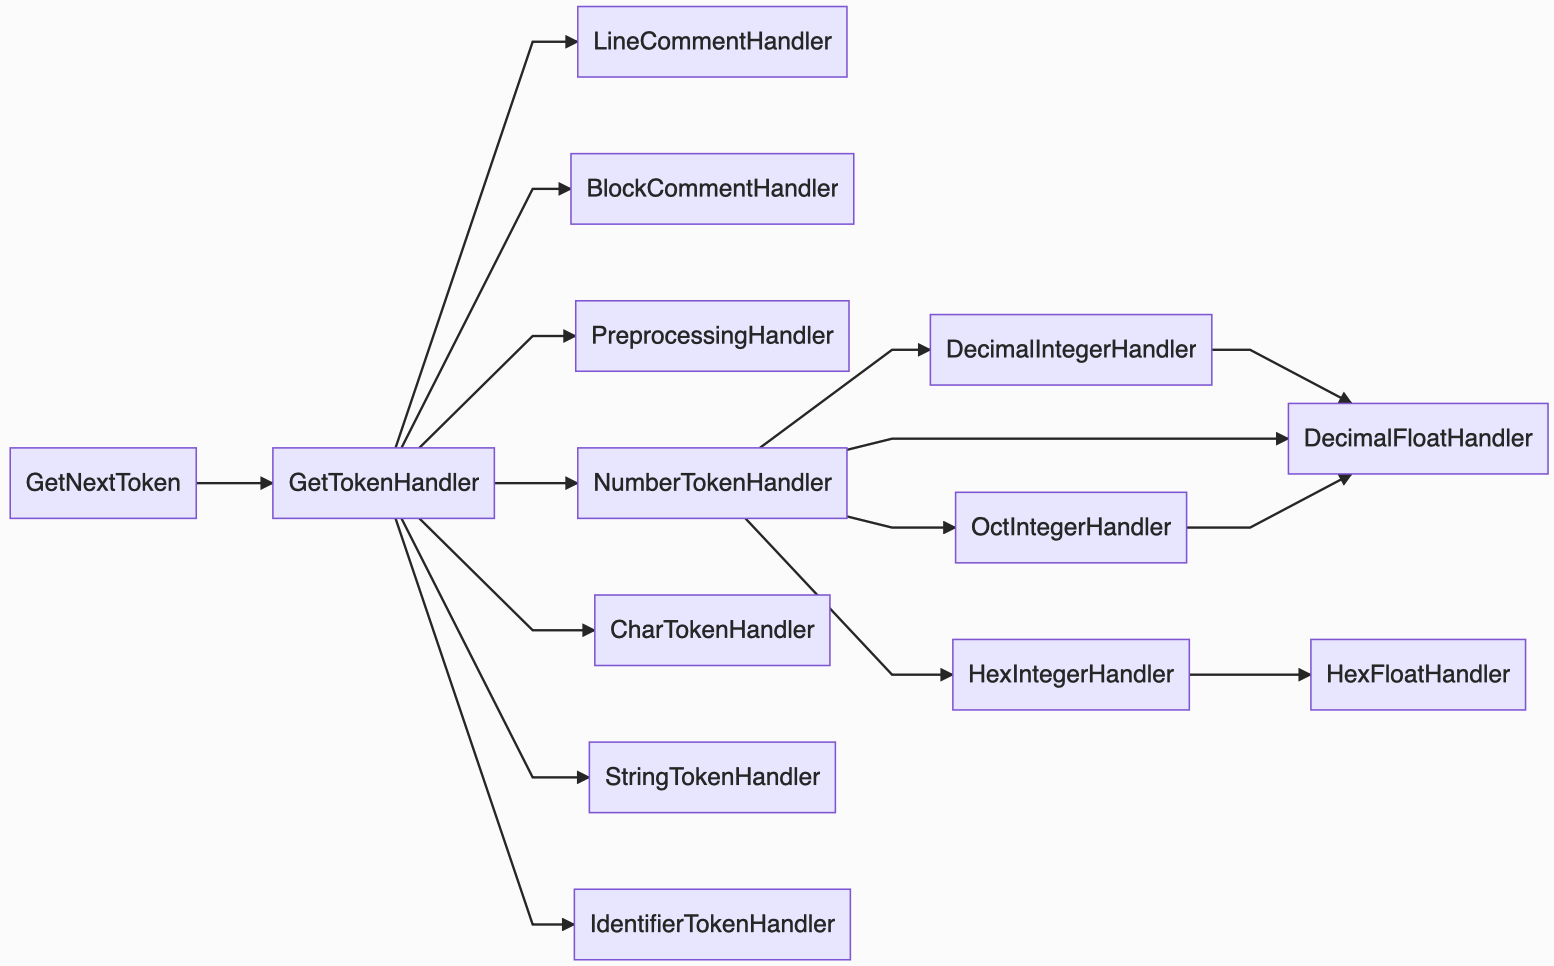
\includegraphics[width=0.9\linewidth]{./images/lexer.png}
    \caption{词法分析器的函数调用关系图\label{fig:lexer}}

\end{figure}

\mintinline{text}{GetNextToken}调用\mintinline{text}{GetTokenHandler}获取下一个记号,并且计数。

\mintinline{text}{GetTokenHandler}中首先跳过所有的空白字符,之后依据符号的类型分别进行处理。

\subsubsection{标点符号处理}

在遇到标点符号时,词法分析器通过向前查看文件流中的字符判断标点符号的类型,此时注意符号的匹配过程是贪心的。例如表达式\mintinline{C}{x+++++y}会被解析为五个记号,依次为\mintinline{C}{x}、\mintinline{C}{++}、\mintinline{C}{++}、\mintinline{C}{+}和\mintinline{C}{y}。

\subsubsection{单行注释处理}

当匹配到符号\mintinline{C}{//}后进入单行注释处理函数\mintinline{text}{LineCommentHandler},此时词法分析器不断读取字符直到行末或者文件末尾。

\subsubsection{块注释处理}

当匹配到符号\mintinline{C}{/*}后进入块注释处理函数\mintinline{text}{BlockCommentHandler},此时词法分析器不断读取字符直到遇到符号\mintinline{C}{*/},如果读到文件末尾,则返回块注释未闭合错误。

\subsubsection{预处理器处理}

当匹配到符号\mintinline{text}{#}时,若该行中此符号前没有非空白字符,则进入预处理器处理函数\mintinline{text}{PreprocessingHandler}。

此后,词法分析器不断读取字符,直到:

\begin{itemize}
    \item 如果遇到换行符或者文件结尾则结束。
    \item 如果遇到\mintinline{C}{\}符号,则跳过该反斜杠后的所有空白字符,如果遇到了换行,则跳过这个换行符号,之后继续预处理器的处理过程。
\end{itemize}

\subsubsection{数字常量处理}

当遇到数字或者符号\mintinline{text}{.}之后的字符是数字时,进入数字常量处理函数\mintinline{C}{NumberTokenHandler}。

\label{numberhandle}数字的处理过程分为两个步骤:第一步,从遇到的第一个符号开始,将所有的数字、大小写字母、紧跟在大小写\mintinline{text}{e}和\mintinline{text}{p}之后的\mintinline{text}{+}和\mintinline{text}{-}符号加入缓冲区中;第二步,判断缓冲区中的数字是否是一个合法数字。

其中,第二步可以调用系统函数\mintinline{C}{stof}完成,但是出于练习目的,我手动实现了判断数字合法性的过程。

通过检查缓冲区的前缀,调用不同的处理函数:

\begin{itemize}
    \item 如果以\mintinline{text}{.}开头,作为十进制浮点数处理。
    \item 如果以\mintinline{text}{0x}或者\mintinline{text}{0X}开头,作为十六进制整数处理。
    \item 如果以\mintinline{text}{0}开头,作为八进制整数处理。
    \item 否则,作为十进制整数处理。
\end{itemize}

\paragraph{十进制整数处理} \mintinline{C}{DecimalIntegerHandler}处理十进制整数。

函数不断向前读取数字,直到:

\begin{itemize}
    \item 读取到缓冲区结束,则返回十进制整数记号。
    \item 读取到\mintinline{text}{.}、\mintinline{text}{e}或者\mintinline{text}{E},则转到十进制浮点数处理。
    \item 读取到其他字符,则判断从当前字符到缓冲区结束的部分是否是合法的整数后缀,如果是,则返回十进制整数记号,否则返回错误。
\end{itemize}

\paragraph{八进制整数处理} \mintinline{C}{OctIntegerHandler}处理八进制整数。

函数不断向前读取八进制数字,直到:

\begin{itemize}
    \item 读取到缓冲区结束,则返回八进制整数记号。
    \item 读取到\mintinline{text}{.}、\mintinline{text}{e}或者\mintinline{text}{E},则转到十进制浮点数处理。
    \item 读取到数字8或者9,则继续向前读取数字,直到遇到\mintinline{text}{.}、\mintinline{text}{e}或者\mintinline{text}{E},则转到十进制浮点数处理,如果读取不到上述三种字符,则返回错误。
    \item 读取到其他字符,则判断从当前字符到缓冲区结束的部分是否是合法的整数后缀,如果是,则返回八进制整数处理,否则返回错误。
\end{itemize}

\paragraph{十六进制整数处理} \mintinline{C}{HexIntegerHandler}处理十六进制整数。

在之前处理十进制数的过程中,我们保证了不存在浮点数小数点前后都没有数字的情况,但是对于十六进制数我们只判断了前缀\mintinline{C}{0x},因此如果十六进制前缀后紧跟一个小数点,需要确保小数点之后至少有一个十六进制字符。如果小数点之后不是十六进制字符,则返回错误。

此外,十六进制数除了前缀和后缀之外至少需要有一位十六进制数字,如果直接读取到非十六进制数字,则返回错误。

函数不断向前读取十六进制字符,直到:

\begin{itemize}
    \item 读取到缓冲区结束,则返回十六进制整数记号。
    \item 读取到\mintinline{text}{.}、\mintinline{text}{p}或者\mintinline{text}{P},则转到处理十六进制浮点数。
    \item 读取到其他字符,则判断从当前字符到缓冲区结束的部分是否是合法的整数后缀,如果是,则返回十六进制整数记号,否则返回错误。
\end{itemize}

\paragraph{十进制浮点数处理} \mintinline{C}{DecimalFloatHandler}处理十进制浮点数。

此函数默认浮点数的整数部分已经处理完成,从小数点或者\mintinline{text}{e}开始处理。

如果有小数点,小数点后可以跟随若干个十进制数字。

如果有\mintinline{C}{e}或者\mintinline{C}{E},其后跟随一个可选的\mintinline{C}{+}或\mintinline{C}{-},之后跟随至少一个十进制数字。

如果此时读取到缓冲区结束,则返回十进制浮点数记号。

否则判断剩余的部分是否是合法的浮点数后缀,如果是,则返回十进制浮点数记号,否则返回错误。

\paragraph{十六进制浮点数处理} \mintinline{C}{HexFloatHandler}处理十六进制浮点数。

此函数默认浮点数的整数部分已经处理完成,从小数点或者\mintinline{text}{p}开始处理。

如果有小数点,小数点后可以跟随若干个十进制数字。

如果有\mintinline{C}{p}或者\mintinline{C}{P},其后跟随一个可选的\mintinline{C}{+}或\mintinline{C}{-},之后跟随至少一个十进制数字。

十六进制浮点数的指数部分是必须的,如果没有指数部分,则返回错误。

如果此时读取到缓冲区结束,则返回十六进制浮点数记号。

否则判断剩余的部分是否是合法的浮点数后缀,如果是,则返回十六进制浮点数记号,否则返回错误。

\subsubsection{字符常量处理}

当读取到符号\mintinline{text}{'}或者字母\mintinline{text}{L}紧跟一个\mintinline{text}{'}时,进入字符常量处理函数\mintinline{text}{CharTokenHandler}。

此后,词法分析器不断读取字符:

\begin{itemize}
    \item 如果遇到\mintinline{text}{'}则结束。
    \item 如果遇到换行符或者文件结尾,则返回未闭合字符常量错误。
    \item 如果遇到\mintinline{C}{\}符号,则读取该反斜杠后的所有空白字符,直到:
    \begin{itemize}
        \item 如果遇到了换行,则跳过这个换行符号,并且丢弃刚才记录到的空白字符,继续字符常量的处理过程。
        \item 否则,将刚才记录到的反斜杠符号和空白字符加入缓冲区,继续字符常量的处理过程。
    \end{itemize}
    \item 否则,将该符号加入缓冲区。
\end{itemize}

\subsubsection{字符串字面量处理}

当读取到符号\mintinline{text}{"}或者字母\mintinline{text}{L}紧跟一个\mintinline{text}{"},进入字符串字面量处理函数\mintinline{text}{StringTokenHandler}。

除了将单引号替换为双引号之外,过程和字符常量处理基本相同。

\subsubsection{标识符处理}

当读取到符号\mintinline{text}{_}或者大小写字母时,进入标识符处理函数\mintinline{text}{IdentifierTokenHandler}。

该函数首先将连续的包含下划线和大小写字母的字符串加入缓冲区中,之后在字典中查找是否存在关键字,如果存在则返回关键字记号,否则返回标识符记号。

\section{用户指南}

在项目目录中执行以下命令来编译:

\begin{code}
\begin{minted}{shell}
mkdir build
cd build
cmake ..
make
\end{minted}
\end{code}

编译完成后,运行:

\begin{code}
\begin{minted}{shell}
./Lexical ../test/test1.txt
\end{minted}
\end{code}

运行截图如\figref{fig:running}所示。

\begin{figure}[htbp]

    \centering
    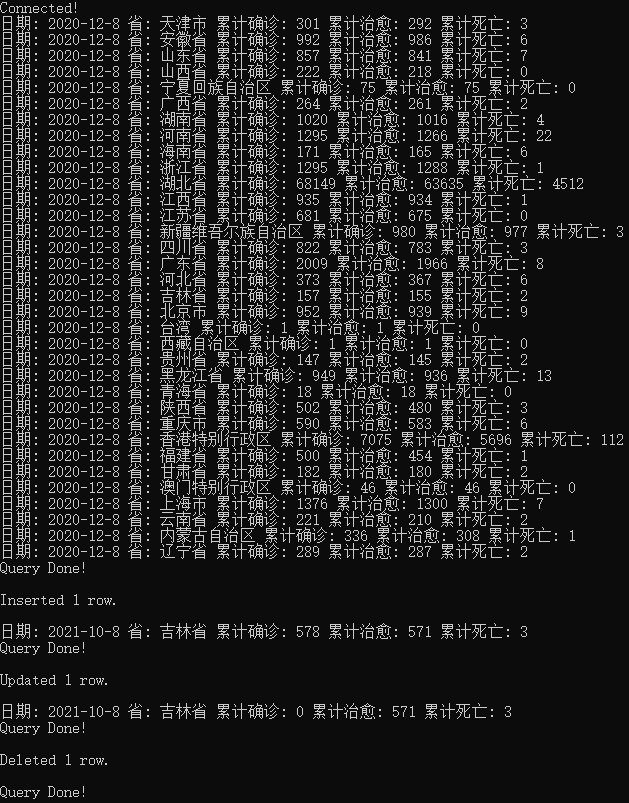
\includegraphics[width=0.7\linewidth]{./Images/running.png}
    \caption{运行截图\label{fig:running}}

\end{figure}

\section{测试结果}

\subsection{测试集1}

此测试集用于简单地测试程序是否正常运行。

\subsubsection{输入}

\begin{code}
\begin{minted}{C}
#include <stdio.h>
int main()
{
    int a, b;
    scanf("%d%d", &a, &b);
    printf("%d\n", a + b);
    return 0;
}
\end{minted}
\end{code}

\subsubsection{输出}

\begin{code}
\begin{minted}{text}
===========Tokens============
[Location] test/test1.txt:1:1
[Type] Preprocessing


[Location] test/test1.txt:2:1
[Type] Keyword
[Value] int

[Location] test/test1.txt:2:5
[Type] Identifier
[Value] main

[Location] test/test1.txt:2:9
[Type] Punctuator
[Value] (

[Location] test/test1.txt:2:10
[Type] Punctuator
[Value] )

[Location] test/test1.txt:3:1
[Type] Punctuator
[Value] {

[Location] test/test1.txt:4:5
[Type] Keyword
[Value] int

[Location] test/test1.txt:4:9
[Type] Identifier
[Value] a

[Location] test/test1.txt:4:10
[Type] Punctuator
[Value] ,

[Location] test/test1.txt:4:12
[Type] Identifier
[Value] b

[Location] test/test1.txt:4:13
[Type] Punctuator
[Value] ;

[Location] test/test1.txt:5:5
[Type] Identifier
[Value] scanf

[Location] test/test1.txt:5:10
[Type] Punctuator
[Value] (

[Location] test/test1.txt:5:11
[Type] String Literal
[Value] %d%d

[Location] test/test1.txt:5:17
[Type] Punctuator
[Value] ,

[Location] test/test1.txt:5:19
[Type] Punctuator
[Value] &

[Location] test/test1.txt:5:20
[Type] Identifier
[Value] a

[Location] test/test1.txt:5:21
[Type] Punctuator
[Value] ,

[Location] test/test1.txt:5:23
[Type] Punctuator
[Value] &

[Location] test/test1.txt:5:24
[Type] Identifier
[Value] b

[Location] test/test1.txt:5:25
[Type] Punctuator
[Value] )

[Location] test/test1.txt:5:26
[Type] Punctuator
[Value] ;

[Location] test/test1.txt:6:5
[Type] Identifier
[Value] printf

[Location] test/test1.txt:6:11
[Type] Punctuator
[Value] (

[Location] test/test1.txt:6:12
[Type] String Literal
[Value] %d\n

[Location] test/test1.txt:6:18
[Type] Punctuator
[Value] ,

[Location] test/test1.txt:6:20
[Type] Identifier
[Value] a

[Location] test/test1.txt:6:22
[Type] Punctuator
[Value] +

[Location] test/test1.txt:6:24
[Type] Identifier
[Value] b

[Location] test/test1.txt:6:25
[Type] Punctuator
[Value] )

[Location] test/test1.txt:6:26
[Type] Punctuator
[Value] ;

[Location] test/test1.txt:7:5
[Type] Keyword
[Value] return

[Location] test/test1.txt:7:12
[Type] Integer Constant
[Value] 0

[Location] test/test1.txt:7:13
[Type] Punctuator
[Value] ;

[Location] test/test1.txt:8:1
[Type] Punctuator
[Value] }

===========Analysis==========
[File Name] test/test1.txt
[Rows] 8
[Characters] 115
[Unknown] 0
[Keyword] 3
[Identifier] 9
[Integer Constant] 1
[Float Constant] 0
[Character Constant] 0
[String Literal] 2
[Punctuator] 19
[Preprocessing] 1
[End Of File] 1
\end{minted}
\end{code}

\subsection{测试集2}

此测试集是一个没有错误的程序,测试了所有关键字、字符、各种类型的常量是否能被正确识别。同时测试了一些略微复杂的数字常量、以及跨行的字符串字面量能否正确识别。

\subsubsection{输入}

\begin{code}
\begin{minted}{C}
#include <stdio.h>
#define LL long long
#define NAME(n)         \
    int name(n)         \
    {                   \
        return name##n; \
    }

typedef struct Node
{
    int a, b;
    long long c;
    union
    {
        float d;
        double e;
    };
    LL f;
} Node;

char ch[10];
enum TT
{
    namea,
    nameb,
};
extern eee;

static int func(unsigned long long var)
{
    var += var * (var - var) + ((var / var) % var);
    unsigned LL *restrict p = &var;
    return var;
}

inline int f()
{
    return sizeof(LL);
}

int main(int argc, char *argv[])
{
    Node node;
    Node *pnode = &node;
    node.a = pnode->a;
    node.b++;
    auto unsigned int x = node.b & ((pnode->c | ch[0]) ^ node.a--);
    volatile unsigned char m = x << 5 + 'c';
    const float y = 3.14, z = 3e5;
    _Bool t = x < z && y > z || x <= y && y >= z;
    node.a = m++ + x;
    _Complex n;
    goto label;
#ifndef what
#define what
#endif
    char *str = "str/*comment*/";
label:
    if (y != z)
        x <<= 2 ^ 3;
    else if (!(x >> 2))
        x >>= 2;
    else
        x &= 5;
    m ^= (x |= ~node.b);
    x -= (node.a *= (m /= (node.b %= 2u)));
    while (1)
    {
        /* This is a loop */
        if (5u)
            break;
        if (y <= z)
            continue;
    }
    do // a comment
    {
        signed _temp = 0x0123456789abcdefUL, temp_temp = 00123251;
        float __ = 0x12f.2p+4;
        switch (_temp)
        {
        case 'd':
            /* Comment
            ???
            @ # `

            break;
            */
            break;

        default:
            break;
        }
    } while (0);
    // a comment "string" 'c' 123321
    for (register int i = 1; i <= -1; ++i)
        ;

    printf("%llu\n", 3ul ? 2llu : 45ull);
    printf("floats \
%f %lf\n",
           1.e-2f, (double).356e+3l);
    return x, 0;
}
\end{minted}
\end{code}

\subsubsection{输出(节选)}

\begin{code}
\begin{minted}{text}
===========Tokens============
[Location] test/test2.txt:1:1
[Type] Preprocessing


[Location] test/test2.txt:2:1
[Type] Preprocessing


[Location] test/test2.txt:3:1
[Type] Preprocessing


[Location] test/test2.txt:9:1
[Type] Keyword
[Value] typedef

[Location] test/test2.txt:9:9
[Type] Keyword
[Value] struct

[Location] test/test2.txt:9:16
[Type] Identifier
[Value] Node

[Location] test/test2.txt:10:1
[Type] Punctuator
[Value] {

[Location] test/test2.txt:11:5
[Type] Keyword
[Value] int

[Location] test/test2.txt:11:9
[Type] Identifier
[Value] a

[Location] test/test2.txt:11:10
[Type] Punctuator
[Value] ,

[Location] test/test2.txt:11:12
[Type] Identifier
[Value] b

[Location] test/test2.txt:11:13
[Type] Punctuator
[Value] ;

[Location] test/test2.txt:12:5
[Type] Keyword
[Value] long

[Location] test/test2.txt:12:10
[Type] Keyword
[Value] long

[Location] test/test2.txt:12:15
[Type] Identifier
[Value] c

[Location] test/test2.txt:12:16
[Type] Punctuator
[Value] ;

[Location] test/test2.txt:13:5
[Type] Keyword
[Value] union

[Location] test/test2.txt:14:5
[Type] Punctuator
[Value] {

[Location] test/test2.txt:15:9
[Type] Keyword
[Value] float

[Location] test/test2.txt:15:15
[Type] Identifier
[Value] d

[Location] test/test2.txt:15:16
[Type] Punctuator
[Value] ;

[Location] test/test2.txt:16:9
[Type] Keyword
[Value] double

[Location] test/test2.txt:16:16
[Type] Identifier
[Value] e

[Location] test/test2.txt:16:17
[Type] Punctuator
[Value] ;

[Location] test/test2.txt:17:5
[Type] Punctuator
[Value] }

...

===========Analysis==========
[File Name] test/test2.txt
[Rows] 103
[Characters] 1847
[Unknown] 0
[Keyword] 61
[Identifier] 100
[Integer Constant] 20
[Float Constant] 5
[Character Constant] 2
[String Literal] 3
[Punctuator] 203
[Preprocessing] 6
[End Of File] 1
\end{minted}
\end{code}

\subsubsection{分析}

通过将输出与输入比较,词法分析器正确地得到了每个记号。

\subsection{测试集3}

此测试集主要测试了合法和非法的字面量能否正确识别,同时将识别结果和gcc的编译结果进行比较。

\subsubsection{输入}

\begin{code}
\begin{minted}{C}
int a[] = {0xe+2, 012823, 123F, 23LU23, 0XFFEUU, 0xU, 0EU, 0x12bufb, 12_, 12g+2, 12p+2};
double b[] = {02582e2, 00.3e-4l, 0X5e5ep2, 0xp0, 3e+l, 0xfpl, 0x5e.2, 2.2.2, 3e5.4, 0e+9U, 0x4h3e-l, .e4, 0xp+2F, 0x.p5L, 5.e+2e-4, 0x.2p+2al};
char c = 'ccc
const char * d = "fff
char a = '\
\end{minted}
\end{code}

\subsubsection{输出(节选)}

\begin{code}
\begin{minted}{text}
===========Tokens============
...

[Location] test/test3.txt:1:12
[Type] Unknown
[Value] Illegal Number 0xe+2

...

[Location] test/test3.txt:1:25
[Type] Punctuator
[Value] ,

[Location] test/test3.txt:1:27
[Type] Unknown
[Value] Illegal Number 123F

...

[Location] test/test3.txt:1:33
[Type] Unknown
[Value] Illegal Number 23LU23

...

[Location] test/test3.txt:1:41
[Type] Unknown
[Value] Illegal Number 0XFFEUU

...

[Location] test/test3.txt:1:50
[Type] Unknown
[Value] Illegal Number 0xU

...

[Location] test/test3.txt:1:55
[Type] Unknown
[Value] Illegal Number 0EU

...

[Location] test/test3.txt:1:60
[Type] Unknown
[Value] Illegal Number 0x12bufb

...

[Location] test/test3.txt:1:70
[Type] Integer Constant
[Value] 12

[Location] test/test3.txt:1:72
[Type] Identifier
[Value] _

...

[Location] test/test3.txt:1:75
[Type] Unknown
[Value] Illegal Number 12g

[Location] test/test3.txt:1:78
[Type] Punctuator
[Value] +

[Location] test/test3.txt:1:79
[Type] Integer Constant
[Value] 2

...

[Location] test/test3.txt:1:82
[Type] Unknown
[Value] Illegal Number 12p+2

...

[Location] test/test3.txt:2:15
[Type] Float Constant
[Value] 02582e2

...

[Location] test/test3.txt:2:24
[Type] Float Constant
[Value] 00.3e-4l

...

[Location] test/test3.txt:2:34
[Type] Float Constant
[Value] 0X5e5ep2

...

[Location] test/test3.txt:2:44
[Type] Unknown
[Value] Illegal Number 0xp0

...

[Location] test/test3.txt:2:50
[Type] Unknown
[Value] Illegal Number 3e+l

...

[Location] test/test3.txt:2:56
[Type] Unknown
[Value] Illegal Number 0xfpl

...

[Location] test/test3.txt:2:63
[Type] Unknown
[Value] Illegal Number 0x5e.2

...

[Location] test/test3.txt:2:71
[Type] Unknown
[Value] Illegal Number 2.2.2

...

[Location] test/test3.txt:2:78
[Type] Unknown
[Value] Illegal Number 3e5.4

...

[Location] test/test3.txt:2:85
[Type] Unknown
[Value] Illegal Number 0e+9U

...

[Location] test/test3.txt:2:92
[Type] Unknown
[Value] Illegal Number 0x4h3e-l

...

[Location] test/test3.txt:2:102
[Type] Punctuator
[Value] .

[Location] test/test3.txt:2:103
[Type] Identifier
[Value] e4

...

[Location] test/test3.txt:2:107
[Type] Unknown
[Value] Illegal Number 0xp+2F

...

[Location] test/test3.txt:2:115
[Type] Unknown
[Value] Illegal Number 0x.p5L

...

[Location] test/test3.txt:2:123
[Type] Unknown
[Value] Illegal Number 5.e+2e-4

...

[Location] test/test3.txt:2:133
[Type] Unknown
[Value] Illegal Number 0x.2p+2al

...

[Location] test/test3.txt:3:1
[Type] Keyword
[Value] char

[Location] test/test3.txt:3:6
[Type] Identifier
[Value] c

[Location] test/test3.txt:3:8
[Type] Punctuator
[Value] =

[Location] test/test3.txt:3:10
[Type] Unknown
[Value] Unclosed Character Constant ccc

[Location] test/test3.txt:4:1
[Type] Keyword
[Value] const

[Location] test/test3.txt:4:7
[Type] Keyword
[Value] char

[Location] test/test3.txt:4:12
[Type] Punctuator
[Value] *

[Location] test/test3.txt:4:14
[Type] Identifier
[Value] d

[Location] test/test3.txt:4:16
[Type] Punctuator
[Value] =

[Location] test/test3.txt:4:18
[Type] Unknown
[Value] Unclosed String Literal fff

[Location] test/test3.txt:5:1
[Type] Keyword
[Value] char

[Location] test/test3.txt:5:6
[Type] Identifier
[Value] a

[Location] test/test3.txt:5:8
[Type] Punctuator
[Value] =

[Location] test/test3.txt:5:10
[Type] Unknown
[Value] Slash Newline at EOF

===========Analysis==========
[File Name] test/test3.txt
[Rows] 5
[Characters] 280
[Unknown] 25
[Keyword] 6
[Identifier] 7
[Integer Constant] 2
[Float Constant] 3
[Character Constant] 0
[String Literal] 0
[Punctuator] 43
[Preprocessing] 0
[End Of File] 1
\end{minted}
\end{code}

\subsubsection{分析}

第一行中的整数常量全部是非法的:

\begin{itemize}
    \item \mintinline{C}{0xe+2}:根据\ref{numberhandle}节说明的两个步骤,\mintinline{C}{0xe+2}会被认为是一个数字常量,而不是分开成三个记号\mintinline{C}{0xe}、\mintinline{C}{+}和\mintinline{C}{2},而根据前缀可以判断这是一个十六进制整数,其中出现\mintinline{C}{+2}的后缀是非法的。
    \item \mintinline{C}{012823}:八进制整数中不应该出现数字8。
    \item \mintinline{C}{123F}:\mintinline{C}{F}不是一个合法的整数后缀。
    \item \mintinline{C}{23LU23}:\mintinline{C}{LU23}不是一个合法的整数后缀。
    \item \mintinline{C}{0XFFEUU}:\mintinline{C}{UU}不是一个合法的整数后缀。
    \item \mintinline{C}{0xU}:十六进制整数必须至少包含一位数字。
    \item \mintinline{C}{0EU}:八进制整数必须至少包含一位数字。
    \item \mintinline{C}{0x12bufb}:\mintinline{C}{ufb}不是一个合法的整数后缀。
    \item \mintinline{C}{12_}:被解析为两个记号\mintinline{C}{12}和\mintinline{C}{_}。
    \item \mintinline{C}{12g+2}:被解析为三个记号\mintinline{C}{12g}、\mintinline{C}{+}和\mintinline{C}{2},其中\mintinline{C}{g}不是一个合法的整数后缀。
    \item \mintinline{C}{12p+2}:被解析为一个记号,但是\mintinline{C}{p+2}不是一个合法的整数后缀。
\end{itemize}

第二行中的浮点数常量只有前三个是合法的:

\begin{itemize}
    \item \mintinline{C}{02582e2}:虽然以0开头并且整数部分出现了数字8,但是是一个合法的十进制浮点数。
    \item \mintinline{C}{00.3e-4l}:同上。
    \item \mintinline{C}{0X5e5ep2}:十六进制浮点数中可以出现多个e。
    \item \mintinline{C}{0xp0}:十六进制浮点数的前缀和指数部分之间至少包含一个十六进制数字。
    \item \mintinline{C}{3e+l}:指数部分至少包含一个数字。
    \item \mintinline{C}{0xfpl}:同上。
    \item \mintinline{C}{0x5e.2}:指数部分不允许出现小数点。
    \item \mintinline{C}{2.2.2}:不能出现多个小数点。
    \item \mintinline{C}{3e5.4}:指数部分不允许出现小数点。
    \item \mintinline{C}{0e+9U}:\mintinline{C}{U}不是一个合法的浮点数后缀。
    \item \mintinline{C}{0x4h3e-l}:指数部分至少包含一个数字。
    \item \mintinline{C}{.e4}:小数点前后至少有一个数字。
    \item \mintinline{C}{0xp+2F}:十六进制浮点数的前缀和指数部分之间至少包含一个十六进制数字。
    \item \mintinline{C}{0x.p5L}:十六进制浮点数的前缀和指数部分之间至少包含一个十六进制数字。
    \item \mintinline{C}{5.e+2e-4}:出现多个指数部分。
    \item \mintinline{C}{0x.2p+2al}:指数部分只能出现十进制数字。
\end{itemize}

第三行和第四行分别是未闭合的字符常量和字符串字面量错误。第五行是通过反斜杠换行后遇到EOF的错误。

\subsection{测试集4}

此测试集主要测试几个转义符号能否正常工作,以及另几个其他类型的错误。

\subsubsection{输入}

\begin{code}
\begin{minted}{C}
%:include<string.h>
int a<::> = <%0, 0%>
const char * str = L"12   \   \      \n\t\v\f      \
sd\"\'";
int main()
<%
    a<:0:> = 1;
    return 0;
%>#include<stdio.h>
/* Unclosed Comment
\end{minted}
\end{code}

\subsubsection{输出(节选)}

\begin{code}
\begin{minted}{text}
===========Tokens============
[Location] test/test4.txt:1:1
[Type] Preprocessing


[Location] test/test4.txt:2:1
[Type] Keyword
[Value] int

[Location] test/test4.txt:2:5
[Type] Identifier
[Value] a

[Location] test/test4.txt:2:6
[Type] Punctuator
[Value] [

[Location] test/test4.txt:2:8
[Type] Punctuator
[Value] ]

[Location] test/test4.txt:2:11
[Type] Punctuator
[Value] =

[Location] test/test4.txt:2:13
[Type] Punctuator
[Value] {

[Location] test/test4.txt:2:15
[Type] Integer Constant
[Value] 0

[Location] test/test4.txt:2:16
[Type] Punctuator
[Value] ,

[Location] test/test4.txt:2:18
[Type] Integer Constant
[Value] 0

[Location] test/test4.txt:2:19
[Type] Punctuator
[Value] }

[Location] test/test4.txt:3:1
[Type] Keyword
[Value] const

[Location] test/test4.txt:3:7
[Type] Keyword
[Value] char

[Location] test/test4.txt:3:12
[Type] Punctuator
[Value] *

[Location] test/test4.txt:3:14
[Type] Identifier
[Value] str

[Location] test/test4.txt:3:18
[Type] Punctuator
[Value] =

[Location] test/test4.txt:3:20
[Type] String Literal
[Value] 12   \   \      \n\t\v\f      sd\"\'

[Location] test/test4.txt:4:8
[Type] Punctuator
[Value] ;

...

[Location] test/test4.txt:7:5
[Type] Identifier
[Value] a

[Location] test/test4.txt:7:6
[Type] Punctuator
[Value] [

[Location] test/test4.txt:7:8
[Type] Integer Constant
[Value] 0

[Location] test/test4.txt:7:9
[Type] Punctuator
[Value] ]

[Location] test/test4.txt:7:12
[Type] Punctuator
[Value] =

[Location] test/test4.txt:7:14
[Type] Integer Constant
[Value] 1

...

[Location] test/test4.txt:9:3
[Type] Unknown
[Value] Unexpected Hash

[Location] test/test4.txt:9:4
[Type] Identifier
[Value] include

[Location] test/test4.txt:9:11
[Type] Punctuator
[Value] <

[Location] test/test4.txt:9:12
[Type] Identifier
[Value] stdio

[Location] test/test4.txt:9:17
[Type] Punctuator
[Value] .

[Location] test/test4.txt:9:18
[Type] Identifier
[Value] h

[Location] test/test4.txt:9:19
[Type] Punctuator
[Value] >

[Location] test/test4.txt:10:1
[Type] Unknown
[Value] Unclosed Comment

===========Analysis==========
[File Name] test/test4.txt
[Rows] 10
[Characters] 186
[Unknown] 2
[Keyword] 5
[Identifier] 7
[Integer Constant] 5
[Float Constant] 0
[Character Constant] 0
[String Literal] 1
[Punctuator] 21
[Preprocessing] 1
[End Of File] 1
\end{minted}
\end{code}

\subsubsection{分析}

词法分析器正确解析出\mintinline{C}{#}、\mintinline{C}{[}等记号,并且正确识别出了换行的字符串字面量和未闭合的块注释。

同时,对于不在行首的预处理器,词法分析器报出了未识别的符号的错误,同时正常解析了其后的\mintinline{C}{include}等记号,这与gcc的表现一致。

\subsection{测试集5}

此测试集主要测试非法符号是否能够识别。

\subsubsection{输入}

\begin{code}
\begin{minted}{C}
`
@
$
##
%:%:
/* ` @ # */
#define \
\end{minted}
\end{code}

\subsubsection{输出}

\begin{code}
\begin{minted}{text}
===========Tokens============
[Location] test/test5.txt:1:1
[Type] Unknown
[Value] Unknown Character `

[Location] test/test5.txt:2:1
[Type] Unknown
[Value] Unknown Character @

[Location] test/test5.txt:3:1
[Type] Unknown
[Value] Unknown Character $

[Location] test/test5.txt:4:1
[Type] Unknown
[Value] Unexpected Hash

[Location] test/test5.txt:5:1
[Type] Unknown
[Value] Unexpected Hash

[Location] test/test5.txt:7:1
[Type] Unknown
[Value] Slash Newline at EOF

===========Analysis==========
[File Name] test/test5.txt
[Rows] 7
[Characters] 37
[Unknown] 6
[Keyword] 0
[Identifier] 0
[Integer Constant] 0
[Float Constant] 0
[Character Constant] 0
[String Literal] 0
[Punctuator] 0
[Preprocessing] 0
[End Of File] 1
\end{minted}
\end{code}

\subsubsection{分析}

对于非法符号,词法分析器能够正确识别,但是注释中的符号会被跳过。

\section{实验总结}

本次实验中我上手编写了一个词法分析程序,使我对词法分析的流程更加清楚,对相关知识点的掌握更加牢固。

为了实现C语言的词法分析,需要有标准的C语言词法规则进行参照,而不是凭感觉编写程序。因此我找到了C99的ISO标准,并且依照标准中定义的词法规则编写程序。标准中对各类记号的文法定义十分清晰,这在一定程度上降低了我编程的难度,但是这其中也有不少细节值得注意。
我在第一次编写过程中出现了不少的疏忽,在多次阅读文法的定义,并且精心设计样例调试的过程中解决了许多bug。

本次实验中我没有完全照搬教材上的实现方式,没有明显地实现一个DFA,也没有明显的状态转移过程,但是我将自动机的思想渗透到了代码中,通过不同的处理函数来实现对不同种类记号的处理。
此外,不同于教材上的缓冲区实现方式,我使用了C++的语法特性,使得维护缓冲区变得更加容易,大大减少编程复杂度。

本次实验除了让我对课内知识有了更多的认识,也使我的C++编程能力和英文文献阅读能力得到提高,我从中收获颇丰。

\end{document}